\chapter{Implementation}

\section{Requirements}
The following requirements are applicable if you choose to run ProConf on your own server.

\begin{itemize}
  \item Apache or other* HTTP server
  \item PHP version 5.3.7 or newer, --with-mysqli --with-mcrypt.\cite{ref5}
  \item MySQL or MariaDB version 5 or newer
  \item 15 MB of disk space for the OpenConf software, plus additional space for submission files
  \item	1 MB of database space per 100 submissions (actual amount will vary based on modules installed, number of reviewers, and other factors)
  \item	The hosting account (web server) will also require:
  \item Create/write access to IITProConf/config.php and IITProConf /data/*
  \item MySQL privileges to: ALTER, CREATE, DELETE, DROP, INSERT, SELECT, TRUNCATE, UPDATE
\end{itemize}

\section{Conference Website}
When Chair  install this system then a website will be created.It is easy to use for chair.Chair can create unlimited menu,dynamically news update,change important date etc.All information for conference will be here.Here some option exist that means make submission,scope and track,news,important date,registration,committees,best paper award etc.Conference website will be helpful for authors,reviewer,chair,track chair.


\begin{figure}[h!]
\centering
  % Requires \usepackage{graphicx}
  
\includegraphics[width=5in,height=3in]{pic/all}
   \caption{Conference website}\label{conference}
\end{figure}




\section{Author’s Section}

\subsection{Author make a submission}
In this section author make a submission easily.He/she will make a  unlimited submission in one account.After make a submission, he/she will upload valuable research paper.
\begin{figure}[h!]
\centering
  % Requires \usepackage{graphicx}
  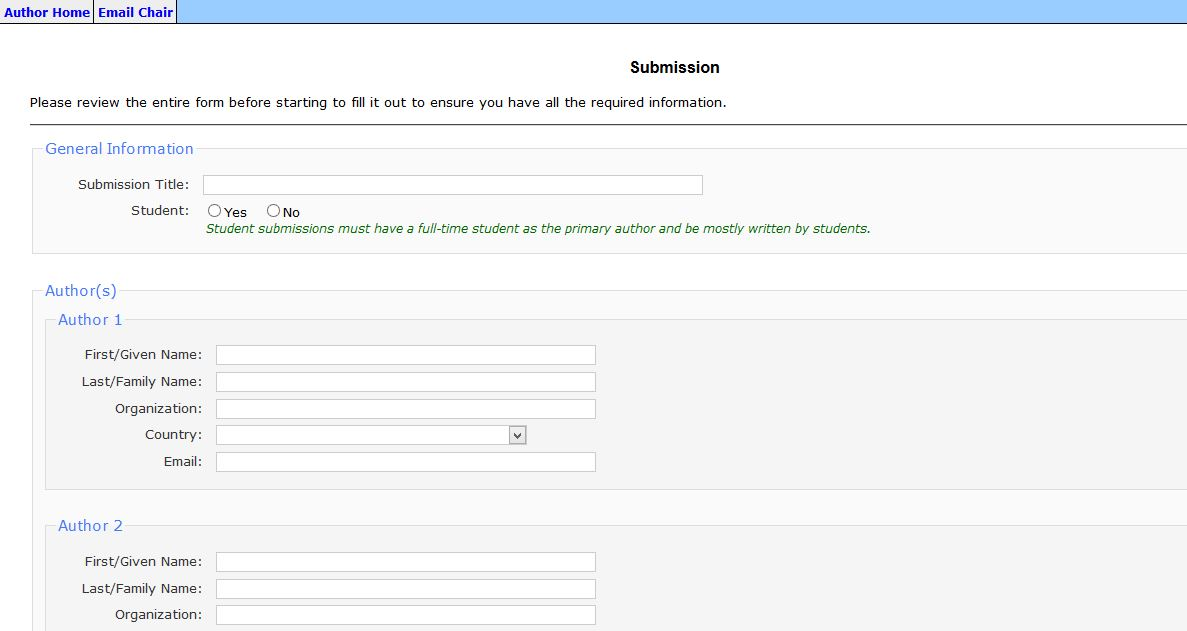
\includegraphics[width=5in,height=3in]{pic/authorm}
   \caption{Author make a submission }\label{authormake}
\end{figure}
\newpage

\subsection{Author home page after submission}
After make a submission then he/she will get a home page.There will be different color exist to easily identify if file not upload,accept or reject paper,pending paper.If chair accept or reject a paper,author will get a notification and a email.If a paper will be accept then author making a camera ready submission.It is very helpful for author for make a submission,upload file,update profile,email chair etc.

\begin{figure}[h!]
\centering
  % Requires \usepackage{graphicx}
  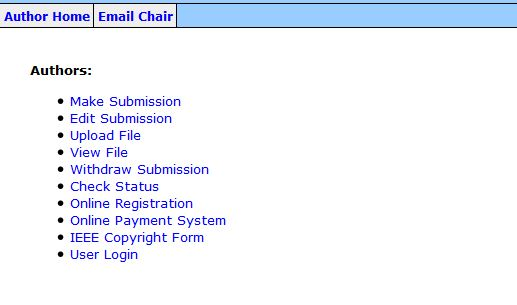
\includegraphics[width=5in]{pic/authorhp}
   \caption{Author home page }\label{authorhome}
\end{figure}



\section{Reviewer home page}
If Chair sign up a reviewer then he/she will get a email for confirmation link.After click a confirmation link as a reviewer,he/she will get a home page.If Chair assign  paper to reviewer,then reviewer will see assign paper.
\begin{figure}[h!]
\centering
  % Requires \usepackage{graphicx}
  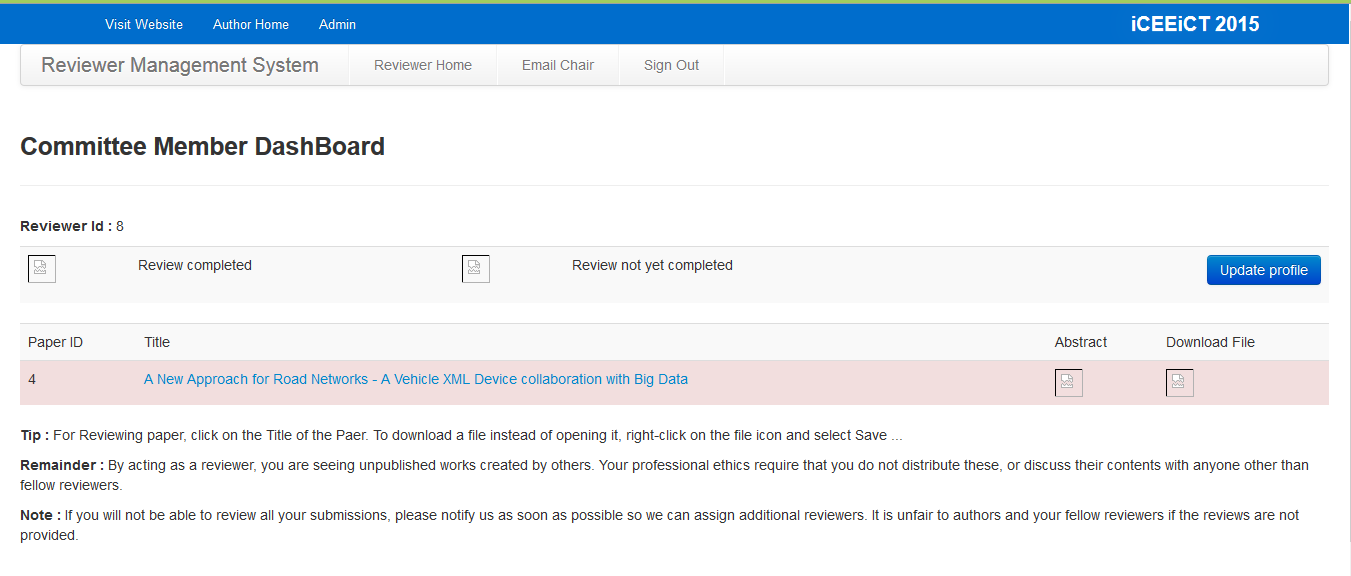
\includegraphics[width=5in]{pic/review1}
   \caption{Reviewer dashboard }\label{review}
\end{figure}



\section{Conference Chair Home Page}
\subsection{Show all paper}
In conference chair home page,chair show the all uploaded paper.There will be different color exist to easily identify if file uploaded or not.

\begin{figure}[h!]
\centering
  % Requires \usepackage{graphicx}
  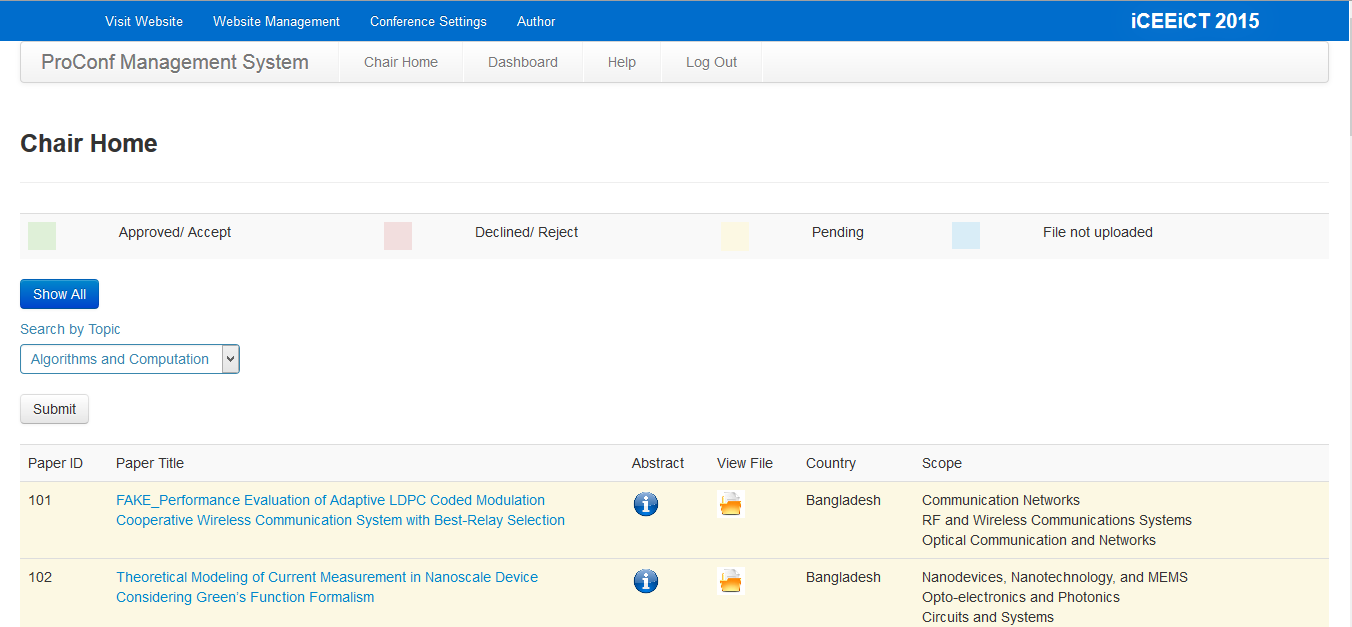
\includegraphics[width=5in,height=2in]{pic/chairhome}
   \caption{Chair home page }\label{chairhome}
\end{figure}


\subsection{ DashBoard}
In conference chair dashboard,chair manage the conference website,pear to pear review system,assign reviewer,accept or reject paper,assign track chair or co-chair or member etc.

\begin{figure}[h!]
\centering
  % Requires \usepackage{graphicx}
  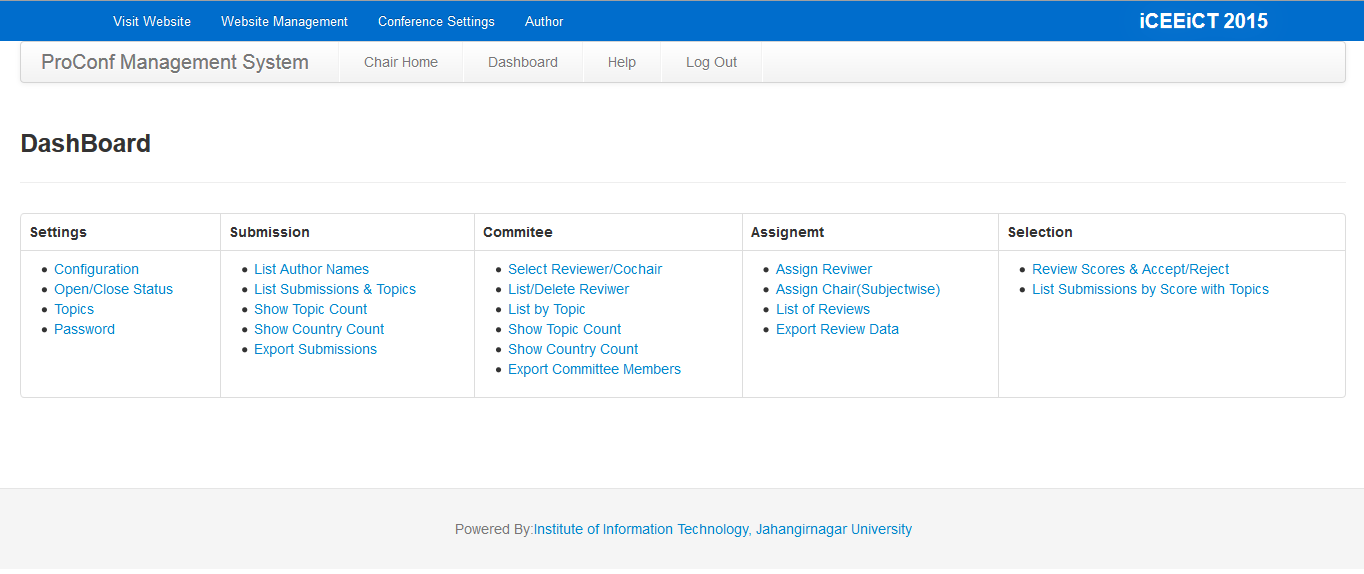
\includegraphics[width=5in]{pic/configuration}
   \caption{Configuration home page }\label{configure}
\end{figure}

\newpage
